\section{Step 1 - Manage Device Memory}
\todo{Opsætning af YAGAL vector type}

\section{Step 2 - Execute .PTX}
\todo{Brug af CUDA driver API}

\section{Step 3 - Make LLC Replacement}
\todo{Generere PTX fra LLVMIR - Bøvlet - derfor - vores llc erstatning! woo}

\begin{figure}[!htb]
    \centering
    \begin{minipage}{.7\textwidth}
        \centering
        \includegraphics[width=0.9\linewidth]{chapters/implementation/figs/LLVMLLC.png}
        \caption{$dt=0.1$}
        \label{fig:prob1_6_2}
    \end{minipage}%
    \begin{minipage}{0.4\textwidth}
        \centering
        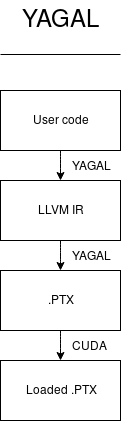
\includegraphics[width=0.5\linewidth]{chapters/implementation/figs/YAGALLLC.png}
        \caption{$dt =$}
        \label{fig:prob1_6_1}
    \end{minipage}
\end{figure}

\section{Step 4 - Generate LLVMIR}
\todo{Lav simpel kernel og brug af vores datatyper}

\section{Step 5 - Multiple functions in one kernel}
\todo{Chaning af functionalitet til en enkelt kernel}

\section{Step 6 - LLVM Optimizations}
\todo{Brug LLVMs erfaring - Det kan betale sig - redegør for det her}

\section{Step 7 - Looping mechanism}
\todo{Behandle data uafhængigt af tråde mængde og input størelse}

\section{Step 8 - Support For Multiple Input Types}
\todo{Support for andre typer end bare floats, så som ints og vectorer}

\section{Final Overview}
\todo{Den "færdige" implementation}